\chapter{Cosmological Solutions of Einstein-Maxwell Theory}
\label{ch:planarem}

In this chapter, we begin our research into planar symmetric solutions by considering Einstein-Maxwell theory as a toy model. We find that the qualitative behaviour for the planar symmetric solutions of the STU model, which are the focus of Chapter \ref{ch:planarstu}, is also found for the simpler, Einstein-Maxwell model. This gives us the great opportunity to discuss some general properties of our cosmological solutions from the perspective of a model we are already familiar with.

The structure of this chapter is as follows. In Section \ref{sec:emsolutions}, we solve the equations of motion, imposing that our solution should be planar symmetric and static. In Section \ref{sec:emcausal}, the causal structure of the solution is studied. In particular, we find that the static ansatz leads to a spacetime region of finite size, where the transverse coordinate is bounded between a singularity and the Killing horizon. Using Eddington-Finkelstein coordinates, we analytically continue through the horizon into a second region in which the metric is time-dependent. As this patch of the spacetime contains the asymptotic region, we call this region the exterior and refer to our solutions as \emph{cosmological solutions}. We study the geodesic motion for null and timelike curves and show that with the exception of transverse null curves, all geodesics are effectively repelled by the singularity. In the static patch of spacetime, we compute the conserved charges and offer a discussion on possible mass-like parameters. In Section \ref{sec:pemglobal}, we consider the global properties of a generalisation of these solutions. We do this in such a way that the discussion covers the solutions of both the Einstein-Maxwell theory and the STU model. For this generalised discussion, we construct Kruskal-like coordinates, and from this, we draw a Penrose-Carter diagram. We then classify the horizons of our cosmological solutions following the work in Section \ref{sec:horizonclassify}, and find that our horizons are past and future \emph{inner horizons}. We conclude this chapter with a discussion of the extremal limit in Section \ref{sec:pemextremal}. We find that for extremal, planar symmetric solutions of Einstein-Maxwell, the spacetime contains a naked singularity.

\section{Planar symmetric solutions}
\label{sec:emsolutions}

We begin this chapter finding planar symmetric, static solutions to the Einstein-Maxwell theory \eq{EMaction}, whose action we repeat for convenience
\begin{equation*}
	S = \frac{1}{16\pi} \int d^4x \sqrt{-g} (-R - F^2).
\end{equation*}
The most general metric ansatz we can make which matches our conditions is given by
\begin{equation*}
   ds^2 = -e^{2F(r)}dt^2 + e^{2H(r)} dr^2 + Y^2(r) (dx^2 + dy^2),
\end{equation*}
where the coordinates take values in
\begin{equation*}
\begin{aligned}
      &x,y,t \in \Real \qquad && r \in [0,\infty).\\
\end{aligned}
\end{equation*}
Our equations of motion are Einstein's equations:
\begin{equation*}
R_{\mu \nu} = -8 \pi T_{\mu \nu},
\end{equation*}
where we have used that the stress-energy tensor is traceless, and Maxwell's equations:
\begin{equation}
   \nabla_\mu F^{\mu \nu} = 0, \qquad \nabla_{[\mu} F_{\nu \rho]} = 0.
\end{equation}
Unlike the Reissner-Nordstr\"om solution studied in Section \ref{sec:rnsol}, we have explicitly assumed our spacetime is static. The main motivation for this is that the following equations simplify when the coordinate dependence is only on the transverse coordinate $r$. We will also assume staticity when solving the equations of motion for planar symmetric solutions of the STU model, and so this allows a similar starting point for both chapters.
 
As in Section \ref{sec:rnsol}, we first compute the stress-energy tensor through considering the form of the gauge fields. Matching our metric ansatz, we will assume the electric and magnetic fields spatially only depend on the transverse direction. We can write them down
\begin{equation*}
   E_r = F_{tr} = \alpha(t,r), \qquad  B_r = \frac{2g_{rr}}{e^{(F+H)}r^2} F_{xy} \quad \Rightarrow \quad F_{xy} = r^2 \beta(t,r),
\end{equation*}
we have chosen the extra factor of $r^2$ in the magnetic field for convenience. From \eq{rnstressenergy}, we can find the form of the stress energy tensor. First calculating,
\begin{equation*}
   F^2 = 2(F_{tr}F_{tr} g^{tt} g^{rr} + F_{xy}F_{xy} g^{xx} g^{yy}) = 2\big(\beta^2 - \alpha^2 e^{-2(F+H)}\big),
\end{equation*}
we find the non-zero components as
\begin{equation*}
   \begin{aligned}
     T_{tt} &= \frac{1}{8\pi} \left( \alpha^2 e^{-2H} + \beta^2 e^{2F} \right), \\
    T_{rr} &=  -\frac{1}{8\pi} \left( \alpha^2 e^{-2F} + \beta^2 e^{2H} \right), \\
    T_{xx} &= T_{yy} = \frac{r^2}{8\pi} \left( \alpha^2 e^{-2(H+F)} + \beta^2\right) .\\
   \end{aligned}
\end{equation*}
To solve Einstein's equations, we need the components of the Ricci tensor. Using \eq{chs}, the non-zero Christoffel symbols are found to be
\begin{equation*}
\begin{aligned}
&\tensor{\Gamma}{^{t}_{tr}} = \partial_r F, \qquad  &&\tensor{\Gamma}{^{r}_{tt}} = e^{2(F-H)}\partial_r F ,\qquad  &&&&\tensor{\Gamma}{^{r}_{xx}}  = \tensor{\Gamma}{^{r}_{yy}} = -e^{-2H} Y \partial_r Y, \\
&\tensor{\Gamma}{^{r}_{rr}} = \partial_r H, \qquad   &&\tensor{\Gamma}{^{x}_{rx}}  = \tensor{\Gamma}{^{r}_{ry}} = \frac{1}{Y} \partial_r Y.
\end{aligned}
\end{equation*}
Substituting these values into \eq{ric}, we obtain the Ricci tensor, all non-zero components are included below
\begin{equation}
\label{eq:riccicomponentspem}
  \begin{aligned}
    R_{tt} &= e^{2(F-H)} \bigg\{ \pardev{F}{r} \bigg( \pardev{H}{r} -  \pardev{F}{r} - \frac{2}{Y} \pardev{Y}{r} \bigg) - \pardev{^2 F}{r^2} \bigg\} ,\\
    R_{rr} &= \pardev{F}{r} \bigg( \pardev{F}{r} - \pardev{H}{r} \bigg) + \pardev{^2F}{r^2} - \frac{2}{Y} \bigg( \pardev{H}{r}\pardev{Y}{r} - \pardev{^2Y}{r^2} \bigg) ,\\
    R_{xx} = R_{yy} &= e^{-2H} \bigg\{ Y\bigg(\pardev{Y}{r}\bigg(\pardev{F}{r} - \pardev{H}{r} \bigg) + \pardev{^2Y}{r^2} \bigg) + \bigg(\pardev{Y}{r}\bigg)^2 \bigg\}.
  \end{aligned}
\end{equation}
As with the spherically symmetric case, by combining the following terms
\begin{equation*}
\begin{aligned}
   0 &= T_{rr} + e^{2(H-F)}T_{tt} = e^{2(H-F)}R_{tt} + R_{rr}, \\
   &= \frac{2}{Y} \bigg\{\pardev{Y}{r} \bigg(\pardev{F}{r} + \pardev{H}{r} \bigg) - \pardev{^2Y}{r^2}\bigg\},
\end{aligned}
\end{equation*}
we obtain a differential equation, which can be solved by picking
\begin{equation*}
	F(r)  = - H(r), \qquad \pardev{^2Y}{r^2} = 0, \quad \Rightarrow \quad Y(r) = A r + B.
\end{equation*}
The integration constants $A,B$ can be absorbed through coordinate transformation: $\{t,r,x,y\} = \{t, r - B, A^{-1}x, A^{-1}y \}$. After making these choices, our line element is in the form
\begin{equation}
   ds^2 = -e^{2F(r)}dt^2 + e^{-2F(r)} dr^2 + r^2 (dx^2 + dy^2).
\end{equation}
From Maxwell's equations, we have that
\begin{equation*}
\begin{aligned}
   &\nabla_t (r^2 F_{tr}) = 0 \quad \Rightarrow  \quad \alpha(t,r) = \alpha(r), \\
   &\nabla_r (r^2 F_{tr}) = 0 \quad \Rightarrow \quad \alpha(r) = -\frac{Q}{r^2},
\end{aligned}
\end{equation*}
Similarly, the Bianchi identity gives:
\begin{equation*}
\begin{aligned}
     &\partial_t F_{xy} = 0 \quad \Rightarrow \quad \beta(t,r) = \beta(r), \\
     &\partial_r F_{xy} = 0 \quad \Rightarrow \quad \beta(r) = -\frac{P}{r^2}.
\end{aligned}
\end{equation*}
The integration constants $Q, P$ are set using Gauss' law, matching with our method Section \ref{sec:rnsol}. However, unlike the Reissner-Nordstr\"om solution, the codimension-two manifold has an infinite surface area, and so conserved charges associated with planar symmetric solutions will be divergent. To work with this, we  consider charge densities per unit coordinate area. Alternatively, we could consider these the total charges contained in a two-torus after compactification of the plane.

With the exact form of the gauge field contribution, we can look at $xx$-component of Einstein's equations
\begin{equation*}
	R_{xx} = -8\pi T_{xx} = -r^2 \left( \frac{Q^2}{r^4} + \frac{P^2}{r^4} \right).
\end{equation*}
The Ricci tensor component can be simplified from the form in \eq{riccicomponentspem} into a total derivative
\begin{equation*}
	R_{xx} =  \partial_r \left( r e^{2F(r)} \right),
\end{equation*}
to obtain the differential equation
\begin{equation*}
	 \partial_r \left( r e^{2F(r)} \right) = - \frac{Q^2 + P^2}{r^2},
\end{equation*}
which can be integrated to 
\begin{equation}
\label{eq:planarsolutionf}
	e^{2F(r)} = \frac{C}{r} + \frac{Q^2 + P^2}{r^2}.
\end{equation}
To ensure the presence of a Killing horizon for the timelike Killing vector $k^\mu = (\partial_t,0,0,0)$, we pick our integration constant $C < 0$ such that $e^{2F(r)}$ has a zero for $r > 0$. We will later find a curvature singularity for $r = 0$ and so allowing $C > 0$, would remove the horizon and the resulting spacetime would contain a naked singularity. For comparison to the Reissner-Nordstr\"om solution, we can write $C = -2M$, for $M > 0$.

In summary, we have found a class of planar symmetric solutions to the Einstein-Maxwell theory, with a line element
\begin{equation}
\label{eq:planareinsteinmaxwell}
\begin{gathered}
	ds^2 = -f(r) dt^2 + \frac{dr^2}{f(r)} + r^2 (dx^2 + dy^2), \qquad f(r) = \left( -\frac{2M}{r} + \frac{e^2}{r^2} \right), \\
	e = \sqrt{Q^2 + P^2}, \qquad \qquad F = -\frac{Q}{r^2} dt \wedge dr + P dx \wedge dy,
\end{gathered}
\end{equation}
parameterised by the integration constants $(M, Q, P)$. However, unlike the Reissner-Nordstr\"om solution, we cannot compare this line element to Newtonian physics by taking the weak field approximation. As a result, we cannot at this point derive a physical interpretation of the integration constant $M$. In the following sections, we will study this line element and its properties and attempt to find a way to properly interpret $M$ from both a gravitational and thermodynamic perspective.

\section{Causal structure}
\label{sec:emcausal}
Studying the metric, we again are interested in the domain of validity of the coordinate system. Like the spherically symmetric solution, the Ricci scalar is zero, but we can compute the Kretschmann scalar\footnote{We used Mathematica for this computation, but SageMath \cite{sagemath} or even pen and paper (and patience) will work.} from the line element and we find
\begin{equation*}
	K = R^{\mu \nu \rho \sigma} R_{\mu \nu \rho \sigma} = \frac{4 \left(3 e^2-2 M r\right)^2}{r^8}.
\end{equation*} 
We see for $r = 0$, as with the spherically symmetric solutions, the Kretschmann scalar diverges indicating the presence of a singularity. Hypersurfaces of constant $r$  will have normal covectors
\begin{equation*}
	n_\mu = (0, dr, 0, 0), \qquad n^2 = - f(r).
\end{equation*}
This shows that the surface for constant $r_h = e^2 / 2M$ will be a null hypersurface. The Killing vector $k^\mu = (\partial_t,0,0,0)$ has a vanishing norm at $r_h$, and so we understand this null hypersurface as a Killing horizon.

During our integration, we explicitly set $M > 0$ to ensure the presence of a Killing horizon. We see that for this patch of spacetime, the function $f(r) > 0$, when the spacelike coordinate $0 < r < r_h$. This is in stark contrast to the spherically symmetric solutions, in which we solved the equations of motion and found ourselves in static regions of spacetime for $r_h < r < \infty$. We find that for these planar solutions to Einstein-Maxwell, imposing that the spacetime should be static, produces a finite static region containing a timelike singularity. We can understand this region as similar to the static region behind the Cauchy horizon $r = r_-$ from the Reissner-Nordstr\"om solution discussed previously (see regions II and IV  in Figure \ref{fig:PenroseRN}).

We note here that we cannot simply say the `asymptotic' region is found when taking the limit to $r \rightarrow \infty$. We will see in Section \ref{sec:4dSolutions}, that this naive limit for the planar solutions of the STU model is just some point in spacetime, which a null curve reaches in finite affine parameter. For the spherically symmetric solutions we discussed, the `asymptotic limit' is defined by the limit in which the Minkowski solution is recovered. As this is not possible for our planar solutions, we instead define the asymptotic limit as the point which takes an infinite affine parameter for a null geodesic to reach. To perform this calculation, we will first need to perform a coordinate transformation to study the spacetime for $r > r_h$.

\subsection{Eddington-Finkelstein coordinates}

To better understand this solution, let us first make an Eddington-Finkelstein coordinate transformation. We do this in the now familiar way, defining a tortoise coordinate $r_\star$ and the ingoing and outgoing null coordinates $v, u$:
\begin{equation*}
	dr_\star = \frac{dr}{f(r)}, \qquad v = t + r_\star, \quad u = t - r_\star,
\end{equation*}
using ingoing coordinates $\{v,r,x,y\}$, we can write the line element
\begin{equation}
\label{eq:planaremef}
	ds^2 = - f(r) dv^2 + 2dv dr + r^2 d\vec{X}^2, \quad f(r) = \left( - \frac{2M}{r} + \frac{e^2}{r^2} \right).
\end{equation}
Notice that now the coordinate range for the transverse coordinate covers all of $0 < r < \infty$. Crossing the horizon for $r = r_h$, the Killing vector $\partial_v$ is spacelike for $r > r_h$. In this new region of spacetime, the transverse coordinate is timelike. 

\subsection{Geodesic motion}
\label{sec:emgeodesics}
Using \eq{planaremef}, we can study the geodesic motion within our spacetime for the full range of $r$. We begin by writing down the Lagrangian of our system
\begin{equation}
    s = - f(r) \left(\diff{v}{\lambda} \right)^2 + 2 \diff{v}{\lambda} \diff{r}{\lambda} + r^2 \left(\diff{x}{\lambda} \right)^2 +r^2  \left(\diff{y}{\lambda} \right)^2 ,
\end{equation}
where $s = \{1, 0, -1\}$ for spacelike, null and timelike geodesics respectively and $\lambda$ is our affine parameter. We compute the constants of motion
\begin{equation*}
	E = - k \cdot u = f(r) \diff{v}{\lambda} - \diff{r}{\lambda}, \qquad a = r^2 \; \diff{x}{\lambda}, \qquad b = r^2 \;\diff{y}{\lambda},
\end{equation*}
which allows us to rewrite the above equation into the form
\begin{equation*}
	\left(\diff{r}{\lambda} \right)^2 = E^2 - V(r), \qquad V(r) = f(r) \left(-s + \frac{a^2 + b^2}{r^2} \right).
\end{equation*}
We have written this in a suggestive way, allowing us to view this as the equation of motion for a particle with mass $m=2$, where we write $V(r)$ to make explicit the interpretation of this function as an effective potential.

First, let us check that $r \rightarrow \infty$ is a suitable limit to describe as the asymptotic region. We consider null, transverse geodesics in which $s = a = b = 0 \Rightarrow V(r) = 0$, and the above equation simplifies to 
\begin{equation*}
	\diff{r}{\lambda} = \pm E \quad \Rightarrow \quad \lambda = \pm \frac{1}{E} \int dr = \pm \frac{1}{E} r \; \bigg|^\infty_{r_0} \; .
\end{equation*}
We see that it will take infinite affine parameter to reach $r \rightarrow \infty$ from some finite point $r_0 > 0$, confirming that $r \rightarrow \infty$ is our asymptotic region. We will discuss the asymptotic structure further in Section \ref{sec:dynamicem}.  

With the above interpretation as the equation of motion of some massive particle, we can study the form of the potential. The domain of validity for the equation of motion is restricted by the inequality
\begin{equation*}
    V(r) \leq E^2.
\end{equation*}
The point at which $V(r_0) = E^2$ is interpreted as the classical turning point of the particle's trajectory. Studying the potential $V(r)$ for the domain of $r$ in the static region, we can look at the paths of causal geodesics.

In Figure \ref{fig:3pot}, we plot $V(r)$ and see that for the static region of our spacetime, the potential is everywhere positive and therefore repulsive. When decreasing $r$ from the horizon towards the singularity, the potential monotonically increases until it diverges in the limit of the singularity. As such, we are guaranteed a unique solution for $V(r_0) = E^2$ within the static region, and hence the existence of a classical turning point.

There is one exception to this: the case when $s = a = b = 0$, specific to transverse null geodesics where the potential is everywhere zero. As a result, our spacetime is not geodesically complete, as transverse null rays will reach the singularity in a finite proper time.

We conclude that for non-zero potentials, a particle will arrive from $\mathcal{J}^-$ and necessarily fall through the horizon at $r = r_h$. The particle will then continue towards the singularity to a minimum distance from the singularity at $r_0$. At this point, it will be reflected and then continue off through the Killing horizon into a second dynamic spacetime, towards $\mathcal{J}^+$. The only causal geodesics which do not follow these trajectories are those for which $V(r)=0$. These are precisely the transverse null geodesics which fall through the horizon from $\mathcal{J}^-$ and straight into the singularity. We can understand this turning point due to the repulsive potential generated by the singularity at $r = 0$.  

\begin{figure}[h!]
\centering
\begin{tikzpicture}[scale=1.5]
 \draw[->] (0,0.6) -- (5,0.6) node[right] {$r$};
 \draw[->] (0,-0.5) -- (0,3) node[above] {$V(r)$};
 
\begin{scope}[shift={(-0.5,0.7)}]
 \draw[domain=0.58:5.45,smooth,variable=\x,blue,thick] plot({\x},{(1 + \x)*(1 - 1.25*\x) / (\x*\x*\x) });
 \end{scope}

\draw[dashed,white!50!black] (.3,2.8) -- (.3,-.5);
\node[left] (one) at (0.8,0.4) {$r_h$};
 \end{tikzpicture}
\caption[Plot of the effective potential for the motion of geodesics for the planar symmetric solution of Einstein-Maxwell theory]{Behaviour of the effective `potential' as a function of $r$ for the set of causal geodesics excluding null transverse geodesics, for which $V=0$. We see that in the static region, for $r < r_h$, the potential is repulsive.}
\label{fig:3pot}
\end{figure}


\subsection*{Proper acceleration}
Seeing that all timelike geodesics reach a classical turning point before reaching the singularity, it is interesting also to study the acceleration of massive particles at rest within the static patch of the spacetime.

Particles at rest follow orbits of the stationary Killing vector field $k^\mu$ with a proper velocity defined by
\begin{equation*}
    u^\mu = \frac{k^\mu}{\sqrt{-k^2}},
\end{equation*}
where the normalisation has been chosen such that $u^2 = -1$. From this, the proper acceleration can be found
\begin{equation}
\label{eq:propacc}
    A^\mu = u^\nu \nabla_\nu u^\mu = \frac{1}{2} \partial^\mu \log(-k^2).
\end{equation}
From the metric \eq{planareinsteinmaxwell}, we can compute the norm of the Killing vector: $k^2 = -f(r)$ to find that
\begin{equation}
\label{eq:properacccomp}
    A^\mu = \half g^{\mu \nu} \partial_\nu \log \left( f(r) \right).
\end{equation}
The only non-zero component of the acceleration is in the transverse direction, and we find
\begin{equation*}
        A^r = \half f(r)
 \partial_r \log \left( f(r) \right)
 = \half \partial_r f(r).
\end{equation*}
Taking the derivative
\begin{equation}
A^r = \frac{2M}{r^2} - \frac{2e^2}{r^3}.
\end{equation}
As the static region is bounded for $0 < r < r_h$, we see that $A^r < 0$ throughout the static patch of the solution. As such, a particle at rest always experiences a force repelling it from the singularity, which matches with our interpretation of a timelike geodesic experiencing repulsion. We remark that the behaviour of geodesics and Killing orbits in our planar symmetric solution is qualitatively the same as for the interior region of the non-extremal Reissner-Nordstr\"om solution behind the Cauchy horizon for $r = r_-$ (regions II and IV in Figure \ref{fig:PenroseRN}). Moreover, in both cases, this static interior region is bounded by horizons both in the past and in the future to regions where the Killing vector field becomes spacelike. 

\subsection{Conserved charges}
\label{sec:emconservedcharges}

\subsubsection*{Electromagnetic charges}
From the line element \eq{planareinsteinmaxwell}, we can compute the conserved charges associated to the Maxwell gauge field. Using the relationship \eq{gausslawcharges} we find
\begin{equation*}
\begin{aligned}
\mathcal{Q} &= \frac{1}{4\pi} \int_{\Real^2} \star F, \\
&= \frac{1}{4\pi} \int_{\Real^2} \sqrt{-g} \epsilon_{trxy} g^{tt} g^{rr} F_{tr} dx \wedge dy, \\
&= \frac{1}{4\pi} \int_{\Real^2} Q dx \wedge dy.
\end{aligned}
\end{equation*}
The integral over the plane $\Real^2$ is divergent. For simplicity in our computations, we parameterise it as
\begin{equation}
\label{eq:pemcharge}
	\mathcal{Q} = \frac{Q \omega}{4\pi}, \qquad \omega = \int_{\Real^2} dx \wedge dy.
\end{equation} 
For the following discussion, we allow $\omega$ to remain explicit in our expressions. However, for the solutions of the STU model presented in Chapter \ref{ch:planarstu}, where there are many more integration constants, we instead consider charge densities by setting $\omega = 1$. Alternatively, we could compactify the plane as a torus, and compute a finite charge by integrating over $T^2$ instead. The conserved magnetic charge is computed in a similar way
\begin{equation*}
\begin{aligned}
	\mathcal{P} &= \frac{1}{4\pi} \int_{\Real^2} F, \\
	&= \frac{1}{4\pi} \int_{\Real^2} \sqrt{-g} F_{xy} dx \wedge dy, \\
	&= \frac{P \omega}{4 \pi}.
\end{aligned}
\end{equation*}

\subsubsection*{Mass}

As discussed in Section \ref{sec:gravitationalmass}, computing the mass in general relativity requires some extra structure. When the solution is static and asymptotically flat, we have a wealth of options which all agree. The Komar energy requires only that the solution is static, but to interpret this as a mass-like quantity, one must have a suitable asymptotic fall off for the solution. The alternative computation comes from the Brown-York mass, which can be defined quasi-locally, but suffers from the necessity to pick the correct background to normalise the result. 

For the planar symmetric solution of Einstein-Maxwell theory, our static region is of finite size. As such, we cannot take an asymptotic limit in the static patch. However, we can still look at mass-like quantities which are position-dependent, following the work of \cite{Burgess:2002vu} in which similar solutions were analysed. In this section, we will compute both a position-dependent Komar mass following Section \ref{sec:komarmass} and a Brown-York quasi-local mass following Section \ref{sec:brownyorkmass}.

The Komar energy is found from \eq{komarenergy}, repeated here
\begin{equation*}
	E_{K} = - \frac{1}{8\pi} \int_{\Real^2} \star dk .  
\end{equation*}
In the static region, where $r < r_h$, the timelike Killing vector field is $k^\mu = \partial / \partial t$. We can compute the exterior derivative and its Hodge-star
\begin{equation*}
	dk = \partial_r f(r) dt \wedge dr, \qquad \star dk =  - \sqrt{-g}  \partial_r f(r) dx \wedge dy, 
\end{equation*}
and so the energy is given by
\begin{equation*}
\begin{aligned}
	E_K &=  \frac{1}{8\pi} \int_{\Real^2} r^2  \partial_r \left( - \frac{2M}{r} + \frac{e^2}{r^2} \right) dx \wedge dy, \\
	&= \frac{\omega}{4\pi} \left(M - \frac{e^2}{r} \right)	.
\end{aligned}
\end{equation*}
Looking at the above result, it is tempting to say that the Komar mass is found by taking the limit $r \to \infty$
\begin{equation}
\label{eq:pemkomar}
	M_K = \lim_{r \rightarrow \infty} E_K = \frac{\omega M}{4\pi} ,
\end{equation}
which when compared to the charges above, looks like the expected value compared to the Reissner-Nordstr\"om solution, and the various factors of $4\pi$ could be removed by allowing $\omega_{S^2} = 4\pi$ to match the integral over the sphere. However, taking this limit, we would we find ourselves in a region where $k^\mu$ is not a timelike Killing vector field, and the original arguments we make for this to be a mass-like parameter are gone. As a result, we have no physical motivation to understand $\lim_{r \rightarrow \infty} E_K$ as a mass-like parameter. We could alternatively think of this as the Noether charge associated to spacelike isometries, and so a form of momentum. However, we do not follow this line of reasoning much further than noting it as an interesting perspective.

In Section \ref{sec:thermopem}, we will use the Euclidean action formalism to derive the thermodynamic internal energy for this solution, and we find that interestingly this calculation matches the naive limit taken above. However, for now, we remain within the static region and save further discussion for later. Notice that for $r < r_h$, the quantity $E_K$ is negative. From this, we can relate the realisation of the position-dependent mass-like parameter being negative to the `repulsive' behaviour of the singularity. However, performing a similar computation in the static region behind the Cauchy horizon for the Reissner-Nordstr\"om solution produces a negative, position-dependent mass. As such, we do not conclude that these static solutions are `negative mass solutions' but rather realise one might say the Reissner-Nordstr\"om solution has an effective negative mass in a particular region.  

We can also compute the Brown-York energy using \eq{BYmass}, repeated here
\begin{equation*}
E_{BY} = -\frac{1}{8 \pi} \int_{\Real^2} \sqrt{\sigma} (\mathtt{k} - \mathtt{k}_0).
\end{equation*}
Looking at the trace of the extrinsic curvature, we see that like the Reissner-Nordstr\"om solution, it is of the form
\begin{equation*}
	\mathtt{k} = \sigma^{\mu \nu} \mathtt{k}_{\mu \nu} = \frac{2 \sqrt{f(r)}}{r},
\end{equation*}
Ignoring the normalisation term $\mathtt{k}_0$, we can write down the Brown-York energy as
\begin{equation*}
\begin{aligned}
	E_{BY} &= -\frac{1}{4 \pi} \int_{\Real^2} r \left(-\frac{2M}{r} + \frac{e^2}{r^2} \right)^{\half}, \\
	 &= -\frac{\omega}{4 \pi} r \left(-\frac{2M}{r} + \frac{e^2}{r^2} \right)^{\half}.
\end{aligned}
\end{equation*}
For the static domain, we have $r < r_h$ and hence $E_{BY} < 0$. However, unlike the Komar energy, taking the limit of $r \to \infty$, we find that $M_{BY}$ is imaginary and so not well defined. This is not too surprising, as we only have a good description for $E_{BY}$ when the spacetime is stationary.

Interestingly, we note a slight variation of this story by instead considering the quasi-local definition for the mass developed by Katz, Lynden, Bell and Israel \cite{Katz_1988}. The Katz-Lynden-Bell-Israel energy differs from the Brown-York quasi-local energy through the introduction of the lapse function $N = \sqrt{f(r)}$ into the expression
\begin{equation*}
E_{KLBI} = -\frac{1}{8 \pi} \int_{\Real^2} \sqrt{\sigma} N (\mathtt{k} - \mathtt{k}_0).
\end{equation*}
In this form, we can compute the energy and find that it is given by
\begin{equation*}
\begin{aligned}
	E_{KLBI} &= -\frac{1}{8 \pi} \int_{\Real^2} r^2 \frac{2f(r)}{r}, \\
	&= - \frac{\omega}{4 \pi} \left( -2M + \frac{e^2}{r} \right),
\end{aligned}
\end{equation*}
and taking the limit, evaluating the boundary at $r \rightarrow \infty$, we find that the energy is real and finite
\begin{equation*}
	M_{KLBI} = \lim_{r \rightarrow \infty} E_{KLBI} = \frac{M \omega}{4 \pi}.
\end{equation*}
However, just like taking the limit for the Komar mass, this moves us into a region where the spacetime is no longer stationary, and the interpretation of the limit as a mass-like quantity is no longer valid. Notice also that like the Komar energy, and the Brown-York energy the Katz-Lynden-Bell-Israel energy is everywhere negative for $r < r_h$.

We note here that we have not included the background contribution associated with $\mathtt{k}_0$. In standard treatments, $\mathtt{k}_0$ is computed by considering the background geometry of the solution. The planar symmetry of our solution means we have no maximally symmetric spacetime asymptotically, and so no natural background geometry to pick. Alternatively, $\mathtt{k}_0$ can be introduced as a counter-term to remove divergences in the energy when considering the asymptotic limit. However, as we have seen, the asymptotic contribution for our solution is finite and so we have no natural choice for a counter-term. We will comment on this again with slightly more detail in Chapter \ref{ch:planarstu} in the context of the planar solution of the STU model. To have confidence in a derived mass-like parameter, we wait until Section \ref{sec:thermopem} where we have the additional structure of a thermodynamic potential to calculate the internal energy, which we derive from the thermodynamic partition function obtained through a modified implementation of the Euclidean action formalism.
 
\subsection{The dynamic region}
\label{sec:dynamicem}

From the line element \eq{planaremef}, we can study the spacetime for which $r > r_h$. Reversing the coordinate transformation, we can write a line element using the coordinates $\{t,r,x,y\}$, valid for $r > r_h$. However, in this region, we have $f(r) < 0$, and the coordinates $t,r$ are spacelike and timelike respectively. For a clearer discussion for the remainder of this chapter, we relabel the coordinates $t \leftrightarrow r$, such that we use the symbol $t$ for the timelike coordinate. In doing this, we are labelling our coordinates with regard to the external region of the spacetime. In this form, we have a line element given by
\begin{equation}
\label{eq:Region_II}
	ds^2 = - \frac{dt^2}{\tilde{f}(t)} + \tilde{f}(t) dr^2 + t^2 d\vec{X}^2, \quad \tilde{f}(t) = \left( \frac{2M}{t} - \frac{e^2}{t^2} \right) \; ,
\end{equation}
where $\tilde{f}(x) = -f(x)$ and the Killing horizon is located for $t = t_h$ such that $\tilde{f}(t_h) = 0$. The line element is valid for $t_h < t < \infty$. 

We see from \eq{Region_II} that the only coordinate dependence of the line element is from the timelike coordinate $t$, and so we understand this as a time-dependent, or \emph{cosmological} solution. The singularity for $t = 0$ is hidden behind a Killing horizon. The horizon itself is a place in time, like the Cauchy horizon for $r = r_-$ in the Reissner-Nordstr\"om solution, which all timelike and null geodesics will inevitably cross. We see that from the static ansatz we began with, the derived planar symmetric solution of the Einstein-Maxwell theory is a cosmological solution containing a Killing horizon. For the remainder of the discussion, we drop the tilde on the function $f(t)$.

We can evaluate the surface gravity of the Killing horizon using the Kodama-Hayward formulation \eq{THK} to find
\begin{equation}
\label{eq:pemsurfacegravity}
	\kappa = -\frac{1}{2} \partial_t f(t_h) = -\frac{4M^3}{e^4},
\end{equation}
which we see is negative. In Section \ref{sec:kruskalgen}, we will study the Kruskal coordinates and the expansions of null geodesics. This will allow for the classification of the trapping horizons for cosmological, planar symmetric solutions we discuss.

Evaluating \eq{Region_II} in the asymptotic limit of $t\rightarrow \infty$, we obtain the line element
\begin{equation}
ds^2 = - \frac{t}{2M} dt^2 + \frac{2M}{t} dr^2 + t^2 d\vec{X}^2 \;,
\end{equation}
which is the `positive mass' version of the planar (type-D) A-III vacuum solution of pure Einstein gravity \cite{Griffiths:2009dfa}. Introducing a new timelike coordinate $t \propto \tau^{2/3}$ and absorbing numerical factors by rescaling $(r,x,y)$, we can write the line element into the form
\begin{equation}
ds^2 = -d\tau^2 + \tau^{-2/3} dr^2 + \tau^{4/3} d\vec{X}^2 \;,
\end{equation}
which belongs to the class of type-D Kasner solutions \cite{Kasner:1921zz}. These are the simplest homogeneous but anisotropic vacuum cosmological solutions of pure Einstein gravity. The A-III/Kasner solution is defined for $0<t,\tau <\infty$ and describes a universe starting in a big bang at $t=\tau=0$, then expanding in the $(x,y)$-directions while contracting in the transverse direction $r$. The Penrose-Carter diagram for the Kasner solution is drawn in Figure \ref{fig:kasnerpc}. Its time-reversed version, given by 
\begin{equation*}
	\begin{aligned}
		ds^2 &= \frac{t}{2M} dt^2 - \frac{2M}{t} dr^2 + t^2 d\vec{X}^2 \;,\;\;\;
&-\infty < t < 0 \;, \\
&=  -d\tau^2 + \tau^{-2/3} dr^2 + \tau^{4/3} d\vec{X}^2\;, \;\;\;\; &-\infty < \tau < 0\;,
	\end{aligned}
\end{equation*}
describes a universe which contracts in the $(x,y)$ directions, expands transversally, and ends in a big crunch at $t=\tau=0$. We then see that the planar solutions describes a bouncing cosmology which interpolates between a contracting and an expanding Kasner cosmology. The presence of the Killing horizon removes the spacelike big crunch and big bang singularities at $t=\tau=0$ and instead introduces an intermediate region containing two timelike singularities. These singularities can be interpreted as sources, and later in Chapter \ref{ch:brane}, we can embed Einstein-Maxwell theory into the STU-supergravity and subsequently into string theory, allowing these source to be identified as brane configurations. 

\begin{figure}[h]
\centering
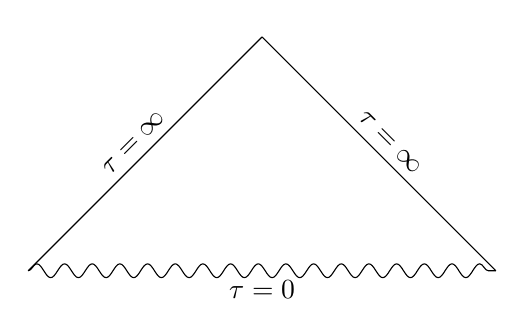
\begin{tikzpicture}[scale = 0.7]
\node (I)  at (0,0)  {};

\path % Four corners of the left diamond
 (I) +(45:-6) coordinate (left)
   +(-45:6) coordinate (right)
   +(0:0) coordinate (top)
   ;
\draw (left) --node[midway, above, sloped] {$\tau=\infty$} (top);
\draw (right) -- node[midway, above, sloped] {$\tau=\infty$} (top);
\draw[decorate,decoration=snake, draw=black] (left) -- node[midway, below] {$\tau=0$}(right);
\end{tikzpicture}
\caption[Penrose-Carter diagram for type-D Kasner solution]{Penrose-Carter diagram for the type-D Kasner solution}
\label{fig:kasnerpc}
\end{figure}


\section{Global structure of planar cosmological solutions}
\label{sec:pemglobal}

In this section, we perform Kruskal-like coordinate transformations which allow us to construct the maximal analytic extensions of the planar symmetric solutions of Einstein-Maxwell. In fact, we will take this opportunity to discuss time-dependent metrics of the form \eq{Region_II}, but leave the form of the function $f(t)$ general. This will allow us to reuse the results from this discussion when we consider the planar symmetric solutions of the STU model, as well as the de Sitter solution in static coordinates, which we introduced in Section \ref{sec:maximallysymmetric} and will revisit as an example in a thermodynamic computation in Section \ref{sec:desitter}.

Obtaining Kruskal-like coordinate systems for these solutions will allow us to understand their global causal structure and to identify the type of all horizons using the classification of trapping horizons reviewed in Section \ref{sec:horizonclassify}. We will find throughout this section only very small departures from the calculations we performed in Section \ref{sec:horizonclassify} for the \sch solution, and so we begin by comparing black hole solutions with a single Killing horizon (\eg the \sch solution) to cosmological solutions with a single Killing horizon (\eg the planar symmetric solutions to Einstein-Maxwell).

The solutions we discuss fall into two categories which are distinguished by the causal relationship between their interior and exterior regions. For all solutions, we call regions {\em exterior} if transverse/radial null geodesics reach a horizon in one direction, but can be extended to infinite affine parameter in the other direction. In terms of our standard transverse/radial coordinate, the asymptotic region is at $r \rightarrow \infty$. In contrast, regions are called {\em interior} regions if transverse/radial null geodesics terminate at a curvature singularity in one direction and reach a horizon in the other. We refer to solutions with a static exterior region as \emph{black hole solutions} and those with a time-dependent exteriors as \emph{cosmological solutions}.  

To properly compare horizons between these solutions, we must set an orientation. We will consider the horizons crossed by future-directed null geodesics which pass from the exterior to the interior region. We pick this convention as this is the horizon one considers for ingoing null curves in the \sch solution, which is crossed by geodesics which start from $\scri^-$ and terminate at the singularity. We will use the static line elements to define ingoing and outgoing null geodesics, fixing the global time orientation of the maximally extended spacetime. Fixing the orientation is important as the extension contains two isometric static regions, where the line element takes the same form in terms of coordinates $(t,r)$, but where the timelike Killing vector field $\partial_t$ is future-directed in one region, but past-directed in the other (where future-directed is defined globally by picking one of the patches to fix the time orientation). 

Starting from a `standard static patch', chosen to fix the definition of ingoing/outgoing and hence the direction of time, we define Kruskal coordinates and obtain a maximally extended spacetime containing four distinct regions. By computing the expansions of null geodesic congruences for each region, we can identify the form of the horizons separating them. Within the context of the thermodynamics we consider in Chapter \ref{ch:triplewick}, we consider future horizons, where the exterior region can causally influence the interior, but not vice versa. The horizons between such regions are  \emph{future outer horizons} for black hole solutions and \emph{future inner horizons} for cosmological solutions. For the thermodynamic formalism based on the Euclidean action that we use in Section \ref{sec:triplewickrotation}, we assume that temperature and surface gravity are related according to \cite{Binetruy:2014ela, Helou:2015zma}, that is, they are proportional. We then find that black holes have positive temperature, while (contracting) cosmologies have negative temperature. 

\begin{figure}
\centering
\begin{subfigure}{.5\textwidth}
  \centering
    \begin{tikzpicture}
    
    \draw[black!15!white] (0,1) -- (5,4);
    \draw[black!15!white] (0,2) -- (5,3);
    \draw[black!15!white] (0,3) -- (5,2);
    \draw[black!15!white] (0,4) -- (5,1);
    \draw[black!15!white] (1,0) -- (4,5);
    \draw[black!15!white] (2,0) -- (3,5);
    \draw[black!15!white] (3,0) -- (2,5);
    \draw[black!15!white] (4,0) -- (1,5);

    % bottom    
    \draw[black!15!white] (2.5,4.1) parabola (4.65,5);
    \draw[black!15!white] (2.5,4.1) parabola (0.35,5);    
    \draw[black!15!white] (2.5,3.75) parabola (4.8,5);
    \draw[black!15!white] (2.5,3.75) parabola (0.2,5);
    \draw[black!15!white] (2.5,3.4) parabola (4.9,5);
    \draw[black!15!white] (2.5,3.4) parabola (0.1,5);

    % top
    \draw[black!15!white] (2.5,0.9) parabola (4.65,0);
    \draw[black!15!white] (2.5,0.9) parabola (0.35,0);    
    \draw[black!15!white] (2.5,1.25) parabola (4.8,0);
    \draw[black!15!white] (2.5,1.25) parabola (0.2,0);
    \draw[black!15!white] (2.5,1.6) parabola (4.9,0);
    \draw[black!15!white] (2.5,1.6) parabola (0.1,0);
    
    % left
    \begin{scope}[shift={(5,0)}, rotate=90]
    \draw[black!15!white] (2.5,4.1) parabola (4.65,5);
    \draw[black!15!white] (2.5,4.1) parabola (0.35,5);    
    \draw[black!15!white] (2.5,3.75) parabola (4.8,5);
    \draw[black!15!white] (2.5,3.75) parabola (0.2,5);
    \draw[black!15!white] (2.5,3.4) parabola (4.9,5);
    \draw[black!15!white] (2.5,3.4) parabola (0.1,5);
    \end{scope}
    
    % right
    \begin{scope}[shift={(0,5)}, rotate=-90]
    \draw[black!15!white] (2.5,4.1) parabola (4.65,5);
    \draw[black!15!white] (2.5,4.1) parabola (0.35,5);    
    \draw[black!15!white] (2.5,3.75) parabola (4.8,5);
    \draw[black!15!white] (2.5,3.75) parabola (0.2,5);
    \draw[black!15!white] (2.5,3.4) parabola (4.9,5);
    \draw[black!15!white] (2.5,3.4) parabola (0.1,5);
    \end{scope}

    \draw[thick, ->] (0,0) -- node[at end, above=0.3cm]{$V$} (5,5);
    \draw[thick, ->] (5,0) -- node[at end, above=0.3cm]{$U$} (0,5);
    
    \draw[thick, red!90!white, ->-]  (2,0) -- (5,3);
    \draw[thick, blue!90!white, ->-]  (5,3) -- (3,5);
    
    \draw[thick, white] (0,0.5) edge  (0,4.5)
         edge[bend right,fill=white, draw=black, thin] node[rotate=90, midway,above, black, font=\fontsize{10}{0}] {$r=\infty$} (0,4.5);
         
    \draw[thick, white] (5,0.5) edge  (5,4.5)
         edge[bend left,fill=white, draw=black, thin] node[rotate=90, midway,below, black, font=\fontsize{10}{0}] {$r=\infty$} (5,4.5);
         
    \draw[thick, white] (0.5,0) edge  (4.5,0)
         edge[bend left,fill=white, draw=black, thin] node[midway,below=0.25cm, black, font=\fontsize{10}{0}] {$r=0$} (4.5,0);
    
    \draw[thick, white] (0.5,5) edge  (4.5,5)
         edge[bend right,fill=white, draw=black, thin] node[midway,above=0.25cm, black, font=\fontsize{10}{0}] {$r=0$} (4.5,5);
         
    \node[rotate=45, font=\fontsize{10}{0}] (a) at (1.5,2) {$t = \infty$};
    \node[rotate=-45, font=\fontsize{10}{0}] (a) at (2,3.5) {$t = -\infty$}; 
        
    \end{tikzpicture}
   \caption{Black hole solutions}
  \label{fig:bhkrus1}
\end{subfigure}%
\begin{subfigure}{.5\textwidth}
  \centering
    \begin{tikzpicture}
    \draw[black!15!white] (0,1) -- (5,4);
    \draw[black!15!white] (0,2) -- (5,3);
    \draw[black!15!white] (0,3) -- (5,2);
    \draw[black!15!white] (0,4) -- (5,1);
    \draw[black!15!white] (1,0) -- (4,5);
    \draw[black!15!white] (2,0) -- (3,5);
    \draw[black!15!white] (3,0) -- (2,5);
    \draw[black!15!white] (4,0) -- (1,5);

    % bottom    
    \draw[black!15!white] (2.5,4.1) parabola (4.65,5);
    \draw[black!15!white] (2.5,4.1) parabola (0.35,5);    
    \draw[black!15!white] (2.5,3.75) parabola (4.8,5);
    \draw[black!15!white] (2.5,3.75) parabola (0.2,5);
    \draw[black!15!white] (2.5,3.4) parabola (4.9,5);
    \draw[black!15!white] (2.5,3.4) parabola (0.1,5);

    % top
    \draw[black!15!white] (2.5,0.9) parabola (4.65,0);
    \draw[black!15!white] (2.5,0.9) parabola (0.35,0);    
    \draw[black!15!white] (2.5,1.25) parabola (4.8,0);
    \draw[black!15!white] (2.5,1.25) parabola (0.2,0);
    \draw[black!15!white] (2.5,1.6) parabola (4.9,0);
    \draw[black!15!white] (2.5,1.6) parabola (0.1,0);
    
    % left
    \begin{scope}[shift={(5,0)}, rotate=90]
    \draw[black!15!white] (2.5,4.1) parabola (4.65,5);
    \draw[black!15!white] (2.5,4.1) parabola (0.35,5);    
    \draw[black!15!white] (2.5,3.75) parabola (4.8,5);
    \draw[black!15!white] (2.5,3.75) parabola (0.2,5);
    \draw[black!15!white] (2.5,3.4) parabola (4.9,5);
    \draw[black!15!white] (2.5,3.4) parabola (0.1,5);
    \end{scope}
    
    % right
    \begin{scope}[shift={(0,5)}, rotate=-90]
    \draw[black!15!white] (2.5,4.1) parabola (4.65,5);
    \draw[black!15!white] (2.5,4.1) parabola (0.35,5);    
    \draw[black!15!white] (2.5,3.75) parabola (4.8,5);
    \draw[black!15!white] (2.5,3.75) parabola (0.2,5);
    \draw[black!15!white] (2.5,3.4) parabola (4.9,5);
    \draw[black!15!white] (2.5,3.4) parabola (0.1,5);
    \end{scope}
    
    \draw[thick, ->] (0,0) -- node[at end, above=0.3cm]{$V$} (5,5);
    \draw[thick, ->] (5,0) -- node[at end, above=0.3cm]{$U$} (0,5);
    
    \draw[thick, red!90!white, ->-] (0,2.5) -- (2.5,5);
    \draw[thick, blue!90!white, ->-] (2.5,0) -- (0,2.5);
    
    \draw[thick, white] (0,0.5) edge  (0,4.5)
         edge[bend right,fill=white, draw=black, thin] node[rotate=90, midway,above, black,  font=\fontsize{10}{0}] {$r=0$} (0,4.5);
         
    \draw[thick, white] (5,0.5) edge  (5,4.5)
         edge[bend left,fill=white, draw=black, thin] node[rotate=90, midway,below, black,  font=\fontsize{10}{0}] {$r=0$} (5,4.5);
         
    \draw[thick, white] (0.5,0) edge  (4.5,0)
         edge[bend left,fill=white, draw=black, thin] node[midway,below=0.25cm, black,  font=\fontsize{10}{0}] {$r=\infty$} (4.5,0);
    
    \draw[thick, white] (0.5,5) edge  (4.5,5)
         edge[bend right,fill=white, draw=black, thin] node[midway,above=0.25cm, black,  font=\fontsize{10}{0}] {$r=\infty$} (4.5,5);
         
    \node[rotate=-45, font=\fontsize{10}{0}] (a) at (3.5,2) {$t = \infty$};
    \node[rotate=45, font=\fontsize{10}{0}] (a) at (3,3.5) {$t = -\infty$}; 
    \end{tikzpicture}
    \caption{Cosmological solutions}
  \label{fig:coskrus}
\end{subfigure}
\caption[Kruskal diagrams for black hole and cosmological solutions]{Kruskal diagrams for black hole and cosmological solutions. Surfaces of constant $r$ are hyperbola and surfaces of constant $t$ are straight lines. Also included are the ingoing (blue) and outgoing (red) null geodesics which are future-pointing.}
\label{fig:kruskalcomp1}
\end{figure}


\begin{figure}[!h]
\centering
\begin{subfigure}{.5\textwidth}
  \centering
  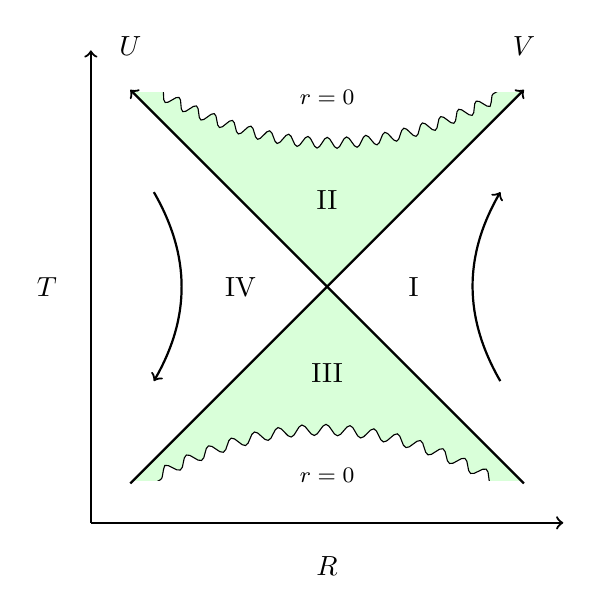
\begin{tikzpicture}
    \fill[green!15!white] (0,0) -- (2.5,2.5) -- (-2.5,2.5);
    
    \fill[green!15!white] (0,0) -- (2.5,-2.5) -- (-2.5,-2.5);
    
    \begin{scope}
    \draw[decoration={snake, amplitude =.7mm, segment length = 2.5mm}, fill=white] 
    decorate {(-2.2, 2.5) to [bend right]  (2.2, 2.5)}
    to (-1.8, 2.5) -- cycle;
    \draw[white, line width=0.25cm] (-2.5, 2.6) --  (2.5, 2.6);
    \end{scope}
    
    \begin{scope}[rotate=180]
    \draw[decoration={snake, amplitude =.7mm, segment length = 3mm}, fill=white] 
    decorate {(-2.2, 2.5) to [bend right]  (2.2, 2.5)}
    to (-1.8, 2.5) -- cycle;
    \draw[white, line width=0.25cm] (-2.5, 2.6) --  (2.5, 2.6);
    \end{scope}
    
    \node (a) at (0, 2.4) {\footnotesize{$r = 0$}};
    \node (a) at (0, -2.4) {\footnotesize{$r = 0$}};
    
    \draw[thick, ->] (-2.5,-2.5) -- node[at end, above=0.3cm]{$V$} (2.5,2.5);
    \draw[thick, ->] (2.5,-2.5) -- node[at end, above=0.3cm]{$U$} (-2.5,2.5);
    
    \draw[thick, ->] (-3,-3) -- node[midway, left=0.3cm]{$T$} (-3,3);
    \draw[thick, ->] (-3,-3) -- node[midway, below=0.3cm]{$R$} (3,-3);
    
    \draw[thick, ->] (-2.2,1.2) to [bend left] (-2.2,-1.2);
    \draw[thick, ->] (2.2,-1.2) to [bend left] (2.2,1.2);    
    
    \node (a) at (1.1,0) {I};
    \node (a) at (-1.1,0) {IV};
    \node (a) at (0,1.1) {II};
    \node (a) at (0,-1.1) {III};
    
    \end{tikzpicture}
   \caption{Black hole solutions}
  \label{fig:sub1}
\end{subfigure}%
\begin{subfigure}{.5\textwidth}
  \centering
  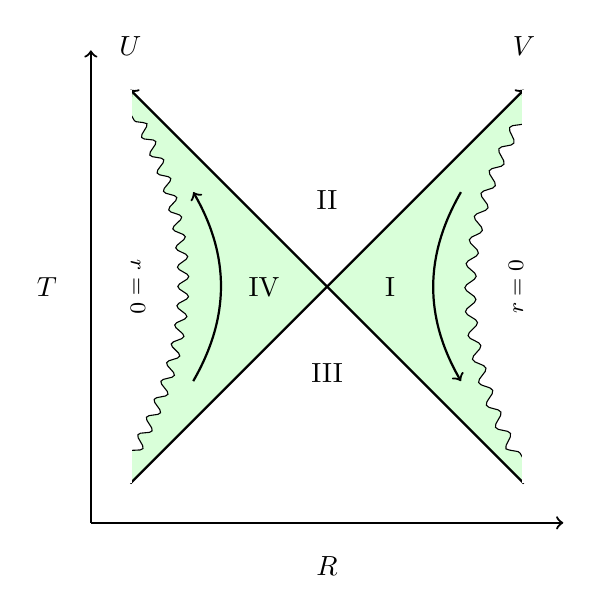
\begin{tikzpicture}
    \fill[green!15!white] (0,0) -- (2.5,2.5) -- (2.5,-2.5);
    
    \fill[green!15!white] (0,0) -- (-2.5,2.5) -- (-2.5,-2.5);
    
    \draw[thick, ->] (-2.5,-2.5) -- node[at end, above=0.3cm]{$V$} (2.5,2.5);
    \draw[thick, ->] (2.5,-2.5) -- node[at end, above=0.3cm]{$U$} (-2.5,2.5);

	\begin{scope} [rotate=90]   
    \begin{scope}
    \draw[decoration={snake, amplitude =.7mm, segment length = 2.5mm}, fill=white] 
    decorate {(-2.2, 2.5) to [bend right]  (2.2, 2.5)}
    to (-1.8, 2.5) -- cycle;
    \draw[white, line width=0.25cm] (-2.5, 2.6) --  (2.5, 2.6);
    \end{scope}
    
    \begin{scope}[rotate=180]
    \draw[decoration={snake, amplitude =.7mm, segment length = 3mm}, fill=white] 
    decorate {(-2.2, 2.5) to [bend right]  (2.2, 2.5)}
    to (-1.8, 2.5) -- cycle;
    \draw[white, line width=0.25cm] (-2.5, 2.6) --  (2.5, 2.6);
    \end{scope}
    \end{scope}
    
    \node[rotate=90] (a) at (2.4, 0) {\footnotesize{$r = 0$}};
    \node[rotate=-90] (a) at (-2.4, 0) {\footnotesize{$r = 0$}};
    
    \draw[thick, ->] (-3,-3) -- node[midway, left=0.3cm]{$T$} (-3,3);
    \draw[thick, ->] (-3,-3) -- node[midway, below=0.3cm]{$R$} (3,-3);
    
    
    \draw[thick, ->] (-1.7,-1.2) to [bend right] (-1.7,1.2);
    \draw[thick, ->] (1.7,1.2) to [bend right] (1.7,-1.2);
    
    \node (a) at (0.8,0) {I};
    \node (a) at (-0.8,0) {IV};
    \node (a) at (0,1.1) {II};
    \node (a) at (0,-1.1) {III};
    
    \end{tikzpicture}
    \caption{Cosmological solutions}
  \label{fig:sub2}
\end{subfigure}
\caption[Comparison of the Kruskal diagrams for black hole and cosmological solutions]{Comparison of the Kruskal diagrams for black hole and cosmological solutions. Shaded regions correspond to the interior regions, curved lines show the direction of the Killing vector field in the static patches of the spacetime.}
\label{fig:comparison}
\end{figure}


\subsection{Kruskal coordinates}
\label{sec:kruskalgen}

We begin by considering the static patch of cosmological solutions which have a line element of the form
\begin{equation}
\label{eq:kruskalgen}
    ds^2 = -f(r) dt^2 + f(r)^{-1} dr^2 + r^2 d\vec{X}^2 ,
\end{equation}
as we saw in Equation \eq{planareinsteinmaxwell}. Later, in Section \ref{sec:cosmologicalsolutionstu}, we will find the STU model has metric of the same form and in Section \ref{sec:desitter}, we will write down the de Sitter solution in static coordinates which is only different in that the two-dimensional line element $d\vec{X}^2$ is instead the metric on $S^2$: $d\Omega^2$. Note that the function $f(r)$ is positive for $r_{\mathrm{sing}} < r < r_h$, and $r_{\mathrm{sing}}$ is the position of the singularity. The domain of $r$ is such that this is the \emph{interior} region of the solution. We assume that $f(r)$ has a simple zero and therefore changes sign at $r=r_h$. Since the Killing vector field $\partial_t$ becomes spacelike for $r>r_h$, the outside region is dynamical. We assume that $f(r)$ is negative for $r_h < r < \infty$, with  $r\rightarrow \infty$ at infinite distance. Thus the horizon at $r=r_h$ is a cosmological horizon. Under the conditions we have imposed on $f(r)$, the surface gravity is \emph{negative}
	\begin{equation*}
	    \kappa = \half \partial_r f(r) \bigg|_{r = r_h} < 0.
	\end{equation*}
As we keep the function general, it will be useful later to use its Taylor expansion near the horizon:
	\begin{equation}
	\label{eq:taylorexpansion}
	        f(r) = 2 \kappa (r - r_h) + \Op((r - r_h)^2) \;.
	\end{equation}

First defining the tortoise coordinate
\begin{equation*}
  r_\star = \int f(r)^{-1} dr, \qquad 0 < r_\star < \infty \;,
\end{equation*}
we introduce future-pointing null coordinates
\begin{equation*}
    v = t + r_\star, \qquad u = t - r_\star, \qquad -\infty < u, v < \infty \;,\;\;\;
    r(v,u) > r_{\mathrm{sing}} \;.
\end{equation*}
Changing to null coordinates, the line element takes the form
\begin{equation*}
  ds^2 = - f(r) dv du + r^2 d\vec{X}^2\;,
\end{equation*}
where $r$ is an implicitly defined function of $r(u, v)$. Note that $v$ is future- and outward-pointing while $u$ is future- and inward-pointing in the interior region. This is the same assignment as in black hole solutions considered in Section \ref{sec:horizonclassify}. With coordinates fixed in this way, we can clearly see what is the difference compared to the static patch of the black hole solutions. Since $r$ points in the opposite direction, the roles of interior and exterior are exchanged, where interior means $r  <r_h$. While $v$ points outwards in both cases, it points away from the horizon for the black hole solutions, but towards the horizon for the cosmological ones. This makes it natural to define Kruskal coordinates such that the standard static region, which we use to fix the overall time orientation, is Region IV, rather than Region I. 

With the region set, we can construct Kruskal like coordinates. We start with the static line element, rewritten using null coordinates $(u, v)$, where $v$ is future-pointing and outward-pointing, while $u$ is future-pointing and inward-pointing, relative to the local coordinates $(t, r)$. This fixes the definitions of the expansion $\theta_\pm$, and the direction of physical time. We define global null Kruskal coordinates $(U, V)$ such that they point in the same direction as $(u, v)$:
\begin{equation*}
\begin{aligned}
    V &= - e^{\kappa v} \qquad & - \infty &< V < 0 \; \;&&\Leftrightarrow \; \; -\infty < v < \infty  \;,\\
    U &= e^{- \kappa u} \qquad & 0 &< U < \infty \; \;&&\Leftrightarrow \; \; -\infty < u < \infty  \;,
\end{aligned}
\end{equation*}
where the factors of the surface gravity have been included to make manifest that the metric is regular at $r=r_h$ where $f(r)$ has its zero. We have also used that $\kappa < 0$. The standard static patch is Region IV, and it is illustrative to compare the black hole case and the cosmological case in Figure \ref{fig:kruskalcomp1} and Figure \ref{fig:comparison}.

The line element in Kruskal coordinates is given by
\begin{equation*}
     ds^2 = - \frac{f(r) e^{-2\kappa r_\star}}{\kappa^2} dV dU + r^2 d\vec{X}^2 \;.
\end{equation*}
We can show this is regular on the horizon using the Taylor expansion \eq{taylorexpansion}
\begin{equation*}
    -2 \kappa r_\star = \int \left( - \frac{2 \kappa  }{2\kappa(r - r_h)} +  \Op(r - r_h) \right) dr  = -\log(r_h - r)  +  \Op((r - r_h)^2)\;,
\end{equation*}
where we note that the choice $\log(r_h - r)$ is made as in the static patch we have $r < r_h$. Putting this together, we obtain
\begin{equation*}
    -f(r) e^{-2\kappa r_\star} = - 2\kappa (r - r_h) e^{-\log(r_h - r)} = 2\kappa + \Op((r - r_h)^2) \;,
\end{equation*}
such that on the horizon, the line element is given by
\begin{equation*}
     ds^2 = \frac{2}{\kappa} dV dU + r_h^2 d\vec{X}^2 \;.
\end{equation*}
In this form, we see that we can extend the Kruskal null coordinates such that
\begin{equation*}
    -\infty < U, V < \infty \;,
\end{equation*}
subject to the constraint that $r(U,V) > r_{\mathrm{sing}}$, where we implicitly write
\begin{equation*}
        U V = - e^{2 \kappa r_\star}, \qquad \frac{V}{U} = -e^{2 \kappa t} \;.
\end{equation*}
The direction of various coordinates in the respective regions is shown in Figure \ref{fig:orientationcos}.

\begin{figure}[!h]
\centering
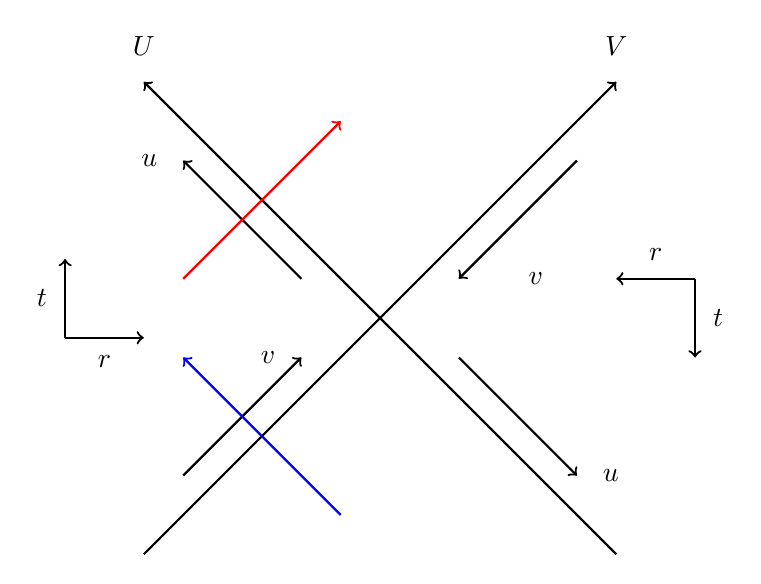
\begin{tikzpicture}

    \draw[thick, ->] (6,0) -- node[at end, above=0.2cm] {$U$} (0,6);
    \draw[thick, ->] (0,0) -- node[at end, above=0.2cm] {$V$} (6,6);
    
    \begin{scope}[shift={(0.5,0)}]
    \draw[thick, ->] (-1.5,2.75) -- node[midway, left=0.1cm] {$t$} (-1.5,3.75);
    \draw[thick, ->] (-1.5,2.75) -- node[midway, below=0.1cm] {$r$} (-0.5,2.75);
    \end{scope}
    
    \begin{scope}[shift={(-0.5,0)}]    
    \draw[thick, ->] (7.5,3.5) -- node[midway, right=0.1cm] {$t$} (7.5,2.5);
    \draw[thick, ->] (7.5,3.5) -- node[midway, above=0.1cm] {$r$} (6.5,3.5);
    \end{scope}
    

    \draw[thick, ->] (2, 3.5) -- node[at end, left=0.2cm] {$u$} (0.5, 5);
    \draw[thick, ->] (0.5, 1) -- node[at end, left=0.2cm] {$v$} (2, 2.5);
        
    \draw[thick, ->, black]  (5.5, 5) -- node[at end, left=-1.2cm, black] {$v$} (4, 3.5);
    \draw[thick, ->, black] (4, 2.5) -- node[at end, right=0.2cm, black] {$u$}(5.5, 1);
    
    \draw[thick, red, ->] (0.5, 3.5) -- (2.5, 5.5);
    \draw[thick, blue, ->] (2.5, 0.5) -- (0.5, 2.5);
\end{tikzpicture}
\caption[Flow of coordinates in the static regions of the Kruskal diagram for cosmological solutions]{Flow of coordinates in the static regions of the Kruskal diagram for cosmological solutions. The red arrow denotes future-directed outgoing null geodesics, the blue arrow denotes future-directed ingoing null geodesics}
\label{fig:orientationcos}
\end{figure}


\subsection{Classification of horizons}
\label{sec:genclassification}
Before we begin, let us precalculate a few useful formulae relating our static coordinates to our Kruskal coordinates
\begin{equation}
\label{eq:drcalc}
    dr = \frac{f(r)}{V U} \frac{1}{2 \kappa} \left( V dU + U dV \right) \;,
\end{equation}
\begin{equation}
\label{eq:dtcalc}
    dt = - \frac{1}{V U} \frac{1}{2 \kappa} \left( V dU - U dV \right) \;.
\end{equation}

To calculate the expansions, we start with the Killing vector field which we can write down in static coordinates as $k  = \pardev{}{t}$. Using the metric tensor, we write down the covector field $k^\flat = -f (r) dt$. From the results above \eq{dtcalc}, we can rewrite the Killing covector field in terms of the Kruskal-like coordinates
\begin{equation*}
    k^\flat = - f(r) dt = \frac{f(r)}{V U} \frac{1}{2 \kappa} \left( V dU - U dV \right) ,
\end{equation*}
with the corresponding vector given by 
\begin{equation*}
    k = \kappa \left(- U \pardev{}{U} + V \pardev{}{V} \right).
\end{equation*}
We now write down the geodesics which are future-pointing within region IV, the standard static region according to our conventions. We pick the normalisation of the covectors to ensure that they are future pointing and pick an overall normalisation for clean results
\begin{equation}
\label{eq:cosnullvec}
    \ell^\flat_{+} = \frac{1}{\kappa} dU, \qquad \ell^\flat_{-} = \frac{1}{\kappa} dV \;,
\end{equation}
or as vectors
\begin{equation*}
    \ell_+ = 2 \kappa \frac{ V U }{f(r)} \left(\pardev{}{V} \right), \qquad \ell_- = 2 \kappa \frac{ V U }{f(r)} \left(\pardev{}{U} \right) \;.
\end{equation*}
We can double check that the normals are future-pointing by computing the inner product of these with the Killing vector field
\begin{equation*}
    k \cdot \ell_+ = -U, \qquad k \cdot \ell_- = V \;,
\end{equation*}
which we see obeys $k \cdot \ell_\pm < 0$ in region IV, where $U > 0$ and $V < 0$. 

Their expansions are calculated following Section \ref{sec:expansionnullhyper}, using \eq{genexpansion}
\begin{equation*}
    \theta_\pm = \nabla_\mu \ell^{\mu}_\pm = \frac{1}{\sqrt{-g}} \partial_\mu \left(\sqrt{-g} \ell^\mu_\pm \right), \qquad \sqrt{-g} = -  \frac{f(r) \sqrt{h}}{V U} \frac{r^2}{2 \kappa^2}\;,
\end{equation*}
where we use that $h = \det \left( r^2 d\vec{X}^2 \right)$ for either the two-sphere or the two-plane depending on the symmetry of the solution. This results in
\begin{equation*}
    \theta_+ = - \frac{4 \kappa}{r} \frac{V U}{f(r)} \pardev{r}{V}, \qquad     \theta_- = - \frac{4 \kappa}{r} \frac{V U}{f(r)} \pardev{r}{U}.
\end{equation*}
To calculate the sign, we use \eq{drcalc} to find that
\begin{equation*}
    \pardev{r}{V} = \frac{f(r)}{V U} \frac{U}{2 \kappa}, \qquad \pardev{r}{U} = \frac{f(r)}{V U} \frac{V}{2 \kappa},
\end{equation*}
such that the expression for the expansions simplifies to
\begin{equation*}
    \theta_+ = \frac{2 U}{r}, \qquad \theta_- = \frac{2 V}{r}.
\end{equation*}
While this already determines the types of all horizons in virtue of knowing the signs for all four regions, we also calculate the Lie derivative at the horizon explicitly. We find that
\begin{equation*}
    \La_{\ell_-} \theta_+ = 2 \kappa \frac{ V U }{f(r)}  \partial_- \left( \frac{2 U}{r} \right) = \frac{4 \kappa}{r} \left( \frac{V U}{f(r)} \right) - \frac{2 V U}{r^2},
\end{equation*}
and on the horizon, we find
\begin{equation*}
    \La_{\ell_-} \theta_+ \bigg|_{r = r_h} = \frac{4 \kappa}{r_h} \cdot \frac{1}{2\kappa} = \frac{2}{r_h}, \qquad     \La_{\ell_+} \theta_- \bigg|_{r = r_h} = \frac{2}{r_h}.
\end{equation*}

Let us look at the left part of the Kruskal diagram, that is, regions III, IV and II (see Figure \ref{fig:sub2}). The physics of the sequence III, I, IV is equivalent but parametrised differently since $\partial_t$ is past-pointing in region I. In region IV of the Kruskal diagram, we have $U > 0$ and $V < 0$. On the horizon given by $V = 0$, we have:
\begin{equation*}
    \theta_+ > 0, \quad \theta_- = 0, \quad \La_{\ell_+} \theta_- > 0,
\end{equation*}
which shows that this is a \emph{past inner horizon}. For the horizon set by $U = 0$, we have that 
\begin{equation*}
    \theta_+ = 0, \quad \theta_- < 0, \quad \La_{\ell_-} \theta_+ > 0,
\end{equation*}
which is a \emph{future inner horizon}. The expansions for all four regions is illustrated in Figure \ref{fig:flipped}. 

\begin{figure}[!h]
\centering
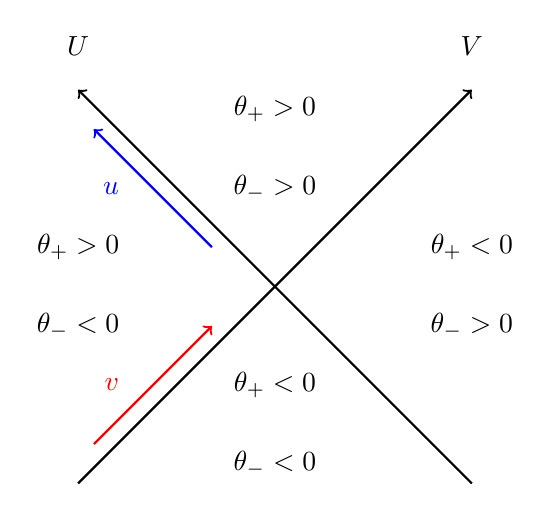
\begin{tikzpicture}

\draw[thick, ->] (-2.5,-2.5) -- node[at end, above=0.3cm]{$V$} (2.5,2.5);
\draw[thick, ->] (2.5,-2.5) -- node[at end, above=0.3cm]{$U$} (-2.5,2.5);

\node (a) at (2.5,0.5) {$\theta_+ < 0$};
\node (a) at (2.5,-0.5) {$\theta_- > 0$};

\node (a) at (-2.5,0.5) {$\theta_+ > 0$};
\node (a) at (-2.5,-0.5) {$\theta_- < 0$};

\node (a) at (0,2.25) {$\theta_+ > 0$};
\node (a) at (0,1.25) {$\theta_- > 0$};

\node (a) at (0,-1.25) {$\theta_+ < 0$};
\node (a) at (0,-2.25) {$\theta_- < 0$};

\draw[thick, ->, blue] (-0.8,0.5) -- node[midway, left=0.3cm] {$u$} (-2.3,2);
\draw[thick, ->, red] (-2.3,-2)-- node[midway, left=0.3cm] {$v$} (-0.8, -0.5);

\end{tikzpicture}
\caption[Signs of the expansions $\theta_\pm$ in the four quadrants of the Kruskal diagram for a cosmological solutions]{Signs of the expansions $\theta_\pm$ in the four quadrants of the Kruskal diagram for a cosmological solution where $\kappa < 0$.}
\label{fig:flipped}
\end{figure}


When considering future-directed causal geodesics which pass through a horizon from the exterior to the interior, we must consider the future inner horizon between region III and region IV. For a future inner horizon, we have that $T_H \propto \kappa < 0$. Later, in Chapter \ref{ch:triplewick}, we will see that this matches with the geometric interpretation of the temperature when we study the first law for the cosmological solutions of this thesis. Overall, the sequence III, IV (or I), II, describes a cosmic bounce, since the solution is a contracting cosmology in III and an expanding cosmology in II. 

\subsection{Penrose-Carter diagram}

From the form of the Kruskal diagram given in Figure \ref{fig:coskrus}, and the Penrose-Carter diagram for the Kasner solution in Figure \ref{fig:kasnerpc}, we can draw the Penrose-Carter diagram for the planar solutions of Einstein-Maxwell. In fact, we will see that this diagram is suitable also for the class of planar symmetric solutions we discuss in Chapter \ref{ch:planarstu}, but more on that later.

The diagram has four regions. Regions II and III are the dynamic regions of the spacetime, with the Kasner spacetime located in the asymptotic limit $t \rightarrow \infty$. A Killing horizon is located at a point in time: $t_h$. All timelike and null geodesics will cross the horizon. Regions I and IV are the static regions, which have a finite size, bounded between $0 < t < t_h$. All causal geodesics, with the exception of null, transverse geodesics, travel to a classical turning point $t_0 > 0$, after which the curve moves with increasing $t$, until it crosses the horizon again. Null transverse geodesics are terminated with finite length once they reach the singularity. After crossing the horizon, all geodesics inevitably travel to a Kasner-like solution for $t \to \infty$.

\begin{figure}[h!]
\centering
\begin{tikzpicture}[scale=1]
\node[above] (0) at (0.13,12) {$i^+$};
\node[below] (1) at (0.13,-4) {$i^-$};
\node (I) at (0,8) {II};
\node (II) at (0,0) {III};
\node (III) at (-2.5,4) {IV};
\node (IV) at (2.5,4) {I};
\path % Four corners of left diamond
 (I) +(90:4) coordinate[label=90:] (IItop)
 +(-90:4) coordinate(IIbot)
 +(0:4) coordinate[label=360:] (IIright)
 +(180:4) coordinate[label=180:] (IIleft)
 ;
\draw (IIleft) --
 node[midway, below, sloped] {$t=\infty, \; r = - \infty$}
 (IItop) --
 node[midway, below, sloped] {$t=\infty, \; r = \infty$}
 (IIright)
     node[midway, above, sloped] {$\mathcal{J}^+$}
           --
 node[midway, above, sloped] {$t = t_h$}
 (IIbot) --
 node[midway, above, sloped] {$t = t_h$}
 (IIleft) -- cycle;

\path % Four conners of the right diamond (no labels this time)
 (II) +(90:4) coordinate (Itop)
 +(-90:4) coordinate (Ibot)
 +(180:4) coordinate (Ileft)
 +(0:4) coordinate (Iright)
 ;
% No text this time in the next diagram
\draw (Ileft) --
 node[midway, below, sloped] {$t = t_h$}
 (Itop) --
 node[midway, below, sloped] {$t = t_h$}
 (Iright) --
 node[midway, above, sloped] {$t=\infty, \; r = - \infty$}
 (Ibot) --
 node[midway, above, sloped] {$t=\infty, \; r = \infty$}
 node[midway, below, sloped] {$\mathcal{J}^-$}
 (Ileft) -- cycle;

%Squiggly lines
\draw[decorate,decoration=snake,draw=black] (Ileft) -- (IIleft)
 node[midway, above, sloped] {$t = 0$};

\draw[decorate,decoration=snake, draw=black] (Iright) -- (IIright)
 node[midway, below, sloped] {$t = 0$};

\draw[blue,dashed,bend right=25, thick] (Ileft) to (Iright);
\draw[blue,dashed,bend right=-25, thick] (Ileft) to (Iright);
\draw[blue,dashed,bend right=25, thick] (IIleft) to (IIright);
\draw[blue,dashed,bend right=-25, thick] (IIleft) to (IIright);
\draw[blue,dashed,bend right=25, thick] (Ileft) to (IIleft);
\draw[blue,dashed,bend right=-25, thick] (Iright) to (IIright);
\draw[->-,orange,bend right=-20, thick] (1) to (0);


\end{tikzpicture}
\caption[Penrose-Carter diagram for our planar symmetric, cosmological solutions]{Penrose-Carter diagram for our planar symmetric, cosmological solutions. Starting in region III, we have a cosmological spacetime with a horizon located at a finite point in time; any observer must necessarily fall through the horizon. Passing through the horizon, the spacetime is static (region IV) with an avoidable (repulsive) naked singularity located at a point in space. Massive particles at rest experience negative acceleration and will leave the static region into a second dynamic spacetime, region II. An example of a complete timelike geodesic is given in orange, spacelike hypersurfaces of constant time are given in blue.}
\label{fig:PC}
\end{figure}



\section{Extremal limit}
\label{sec:pemextremal}
Let us briefly discuss the extremal limit for this class of planar solutions. We found in \eq{pemsurfacegravity} that the surface gravity is negative and equal to
\begin{equation*}
	\kappa = - \frac{4M^3}{e^4}.
\end{equation*}
In the spherically symmetric solutions, we found that $\kappa \to 0$ when we allowed the mass and charge to be equal: $M \to e$. For this solution, we see that in this limit the surface gravity will remain finite. Instead, by taking the limit $M \rightarrow 0$, the surface gravity vanishes and the line element for this solution is given by
\begin{equation*}
	ds^2 = \frac{t^2}{e^2} dt^2 - \frac{e^2}{t^2} dr^2 +  t^2 \left( dx^2 + dy^2 \right).
\end{equation*}
The resulting spacetime has $t,r$ spacelike and timelike respectively, and so we see the extremal limit produces a static solution with a naked, timelike singularity located at $t = 0$. 

For the non-extremal solution, the horizon was located for 
\begin{equation*}
	t_h = \frac{e^2}{2M},
\end{equation*}
and so we can understand the limit of $M \to 0$ as pushing the horizon location off to infinity. This results in changing the causal structure such that the dynamic region is lost and only the static patch of spacetime remains, with the singularity left exposed. In terms of catchy phrases for a presentation, one could say that the extremal limit undresses the solution.

\begin{figure}[h]
\centering
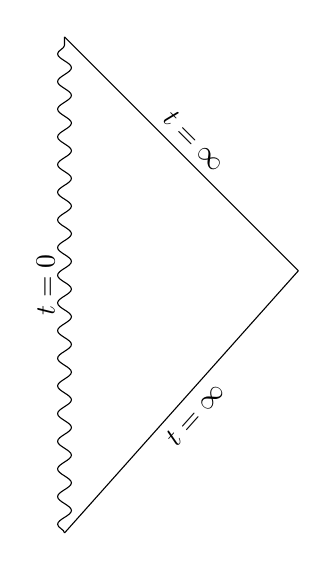
\begin{tikzpicture}[scale = 0.7]
\node (I)  at (0,0)  {};
\path % Four corners of left diamond
 (I) +(90:-9) coordinate (bottom)
   +(-45:6) coordinate (right)
   +(0:0) coordinate (top)
   ;
\draw (top) --node[midway, above, sloped] {$t=\infty$} (right);
\draw (right) -- node[midway, below, sloped] {$t=\infty$} (bottom);
\draw[decorate,decoration=snake, draw=black] (bottom) -- node[midway, sloped, above] {$t=0$}(top);	
\end{tikzpicture}
\caption[Penrose-Carter diagram for extremal planar symmetric solution of the Einstein-Maxwell theory]{Penrose-Carter diagram for extremal planar symmetric solution of the Einstein-Maxwell theory.}
\label{fig:PCextremalplanarem}
\end{figure}

Relabelling coordinates such that $t \leftrightarrow r$ and absorbing the constant $e$, we can write the extremal line element into the form
\begin{equation*}
	ds^2 = - \frac{dt^2}{r^2} + r^2 \left(dr^2 + dx^2 + dy^2 \right).
\end{equation*}

\section{Discussion}

In this chapter, we began our study on planar symmetric solutions of general relativity by considering Einstein-Maxwell theory. This is a particularly interesting starting point, as not only does it allow us to directly compare our solutions with the well known Reissner-Nordstr\"om solutions, we will also see in Section \ref{sec:emfromstu}, that we recover the Einstein-Maxwell Lagrangian through enforcing that the scalar fields are constant for the $\N = 2$ supergravity solutions we consider in the next chapter. This allows for a comparison between the simpler solution discussed in this chapter to the more complicated supergravity solution which follows.

When solving the equations of motion, we assumed that the spacetime was both static and planar symmetric. We saw in Equation \eq{planarsolutionf} that the resulting spacetime metric contained either a Killing horizon or a naked singularity, depending on our choice of sign for the integration constant $C$. Unlike spherically symmetric solutions, we cannot compare our asymptotic geometry to the Newtonian limit and as such we set the sign by hand, ensuring the presence of a Killing horizon by picking $C < 0$. This is beneficial in that it avoids violating cosmic censorship, but it is also in our interest as we wish to better understand the structure of planar symmetric Killing horizons.

The surprising result of these planar symmetric solutions is that despite enforcing that the solution was static, the resulting spacetime metric describes a finite region of spacetime in which the transverse coordinate is bounded between a curvature singularity and the Killing horizon. Analytically continuing through the horizon, we reach a new patch of spacetime which is time-dependent with an asymptotic geometry which is that of the type-D Kasner spacetime. We refer to this region as \emph{exterior} as it contains the asymptotic region, and so we understand the planar symmetric solution as a cosmological solution, and the Killing horizon as a cosmological horizon.

Studying the static region, we saw that the spacetime is geodesically complete for timelike geodesics, which instead of reaching the singularity, reach some minimum distance before being repelled. The only geodesics which reach the singularity in finite affine parameter are null, transverse geodesics. The repulsive interpretation of the singularity within the static region is further justified as massive particles at rest experience a negative proper acceleration, and the position-dependent mass quantities are negative. We can compute the surface gravity of the horizon, which we find is negative and vanishes in the limit $M \to 0$. In the extremal limit, the location of the horizon is pushed off to infinity and the resulting spacetime is everywhere static, with a naked singularity. Considering the Penrose-Carter diagram in Figure \ref{fig:PC}, we can think of this extremal limit as setting the volumes of the dynamic regions to zero as the horizon is moved off to asymptotic infinity. 

The main result of this chapter is the generalised discussion of the causal structure of cosmological solutions containing a single horizon. By considering the static patch of the cosmological solutions for line elements which are of the form
\begin{equation*}
	ds^2 = - f(r) dt^2 + f(r)^{-1} dr^2 + g(r) d\vec{X}^2,
\end{equation*}
where $d\vec{X}^2$ can be either the metric for the two sphere, or the plane and $f(r)$ has one zero, we can write down the line element in terms of Kruskal-like coordinates. This allows us to then find the Penrose-Carter diagram and the classification of the trapping horizons for the solutions in this chapter, but also for the planar symmetric solutions of the STU model, and for the de Sitter solution, which is used as an example in Section \ref{sec:desitter}. We will come back to this solution in Chapter \ref{ch:triplewick} when we consider the thermodynamics of the Killing horizon, and it will appear again in our concluding remarks, when in Section \ref{sec:furtherwork}, we discuss an ongoing project that attempts to classify a larger set of dual solutions, of which the planar symmetric solutions of Einstein-Maxwell are included.
